\documentclass[ngerman]{fbi-aufgabenblatt}

% Folgende Angaben bitte anpassen

\renewcommand{\Vorlesung}{GSS}
\renewcommand{\Semester}{SoSe 2018}

\renewcommand{\Aufgabenblatt}{1}
\renewcommand{\Teilnehmer}{Knudsen, Rasch, Runge, Titov}

\usepackage{url}
\usepackage{listings}
\usepackage[]{graphicx}

\begin{document}

%
% Aufg. 1
%
\aufgabe{Allgemeine Aussagen zur IT-Sicherheit}

% 1.1
\textbf{1.1 Verteilte Systeme (optional)}

\dq Ein Verteiltes System (VS) ist eine durch ein Kommunikationssystem lose gekoppelte Menge von Knoten, wobei

\begin{itemize} 
\item die Knoten kooperieren, um Systemfunktionen auszuführen (verteilte systemweite Kontrolle)
\item keine zwei Prozesse dieselbe Sicht des Systemzustands besitzen und insbesondere kein zentraler Prozess existiert, 
     der andere Prozesse mit einer konsistenten, identischen Sicht des globalen Systemzustands versorgen kann.\dq
\end{itemize}

(Quelle: Prof. Dr. rer. nat. Bernd E. Wolfinger - Datenkommunikation und Rechnernetze (DKR) Skript, S. 15)

\dq Die 3 wichtigsten Aspekte eines verteilten Systems sind:

\begin{itemize} 
\item lose gekoppelte Knoten (kein gemeinsamer Speicher; Kommunikation nur durch Nachrichten)
\item verteilte systemweite Kontrolle
\item kein globaler Systemzustand\dq
\end{itemize}

(Quelle: Prof. Dr. rer. nat. Bernd E. Wolfinger - Datenkommunikation und Rechnernetze (DKR) Foliensatz 1, Folie 44)

3 Beispiele für verteilte Systeme:
\begin{itemize} 
\item Terminalnetze (bestehend aus Terminals und Terminalkonzentratoren)
\item Mobile Systeme (bestehend z.B. aus Endgerät und Peripherie-Komponenten wie Kamera, Drucker, Wifi-Festplatte,...)
\item ein beliebiger Abschnitt des Internets, der aus mehr als einem Rechner besteht
\end{itemize}

% 1.2
\textbf{1.2 Sicherheit verteilter Systeme (optional)}

Vorteile: 
\begin{itemize}
\item Wenn ein Verteiltes System mit Verfügbarkeitsverbund vorliegt, kann nach einem erfolgreichem Angriff auf einen Knoten die Funktionalität des Gesamtsystems weiterhin gewährleistet werden. 
\item Wenn ein Verteiltes System mit Datenverbund vorliegt, kann nach einem erfolgreichem Angriff auf einen Knoten mit einhergehendem Datenverlust die Verfügbarkeit der Daten durch einen  anderen Knoten weiterhin gewährleistet werden.
\item ...
\end{itemize}

Nachteile: 
\begin{itemize}
\item Durch Infektion eines Rechners können die anderen Rechner des verteilten Systems leichter infiziert werden, u.a. da zwischen ihnen regelmäßig Nachrichten ausgetauscht werden
\item Umfang der Sicherheitsvorkehrungen und Einfachheit des Zugriffs stehen in Konkurrenz zu einander
\item ...
\end{itemize}

% 1.3
\textbf{1.3 Ursachen (Pflicht, 6 Punkte)}

Vermutungen:

\begin{itemize} 
\item Kosten
\item Unwissen
\item Fahrlässigkeit
\end{itemize}

Tatsächlich eher: 

\begin{itemize} 
\item Defizite in der Zusammenarbeit von IT und Sicherheitsverantwortlichen
\item Mangelnde oder mangelhafte Sicherheitskonzepte für neue Technologien (z.B. Mobile Endgeräte, Cloud, ...)
\item Mangel an Collaboration und Ressourcen
\end{itemize}

\begin{itemize} 
\item immer mehr verwundbare Endpunkte, 
\item unwirksame Strategien in der technologischen Implementierung und organisatorischen Priorisierung von IT-Sicherheit 
\item sowie die Unfähigkeit, Mitarbeitern Best Practices nahezubringen.
\end{itemize}

(Quelle: \url{https://www.ponemon.org/local/upload/file/Third_Annual_Study_Patient_Privacy_FINAL.pdf})

Referenzen: 
Studien, z.B. von <kes> – Die Zeitschrift für Informations-Sicherheit, die Microsoft-Sicherheitsstudien, 
oder auch die oben verlinkte Studie vom Ponemon Institute.

Komplikationen: 
\begin{itemize}
\item Unternehmen werden unter Umständen nicht dran interessiert sein,
Probleme ihres Umgangs mit IT-Sicherheit zu offenbaren, zumal der Punkt \dq Unwissen\dq \ die kritische Auseinandersetzung damit erschwert bzw. evtl. sogar unmöglich macht.
\item Studien werden evtl. durch die Auftraggeber oder die Durchführenden selbst insofern kompromittiert, als dass die dargestellten Ergebnisse nicht (ganz) der Realität entsprechen.
\item Befragte haben schlichtweg keine Fachkentnisse und bieten somit ein verzerrtes Bild der Realität.
\end{itemize}

% 1.4
\textbf{1.4 Digitale Signaturen (optional)}

Im Gegensatz zu einer Signatur im Sinne einer physischen Unterschrift mit Stift auf Papier handelt es sich
\dq bei der digitalen Signatur (DSig) [...] um einen asymmetrischen elektronischen Schlüssel, 
der die Identität des Benutzers sicherstellt. Der Schlüssel wird mit dem privaten Schlüssel des Absenders verschlüsselt 
und vom Empfänger mit dem öffentlichen Schlüssel gelesen.\dq

(Quelle: \url{https://www.itwissen.info/Digitale-Signatur-digital-signature-DSig.html})


%
% Aufg. 2
%
\aufgabe{Schutzziele}

% 2.1
\textbf{2.1 Abgrenzung I (Pflicht, 14 Punkte)}

a) Anonymität, Pseudonymität und Unbeobachtbarkeit

Während die Identität eines Akteur bei gewahrter \emph{Anonymität} lediglich nicht preisgegeben wird,\\
wird bei \emph{Pseudonymität} eine falsche Identität vorgeschoben, wobei die wahre Identität bei Eintritt besonderer Rahmenbedingungen ermittelt werden kann,\\
und bei \emph{Unbeobachtbarkeit} ist weder seine wahre, noch eine vorgetäuschte Identität ersichtlich. Seine Handlungen können nicht beobachtet werden oder es kann nicht festgestellt werden, dass die Handlungen einem einzelnen Akteur zuzuordnen sind.  

b) Vertraulichkeit und Verdecktheit

Während bei \emph{Vertraulichkeit} die Daten eines Akteurs vor Blicken Dritter geschützt sind,

ist bei \emph{Verdecktheit} das Wissen über das Stattfinden einer Übertragung an sich vor Dritten geschützt.

c) Integrität und Zurechenbarkeit

Bei \emph{Integrität} wird versucht, eine Veränderung der Daten zu verhindern, 

während bei \emph{Zurechenbarkeit} die Veränderung der Daten einem Akteur nachgewiesen werden kann.

% 2.2
\textbf{2.2 Techniken (optional)}


\newpage
\aufgabe{Angreifermodell}
% Aufg. 3

% 3.1
\textbf{3.1 Angreifermodell (optional)}

Das Angreifermodell definiert die maximal berücksichtigte Stärke eines
Angreifers, gegen den ein Schutzmechanismus gerade noch wirkt.

Es beschreibt:
\begin{itemize}
\item Rollen des Angreifers (Außenstehender, Benutzer, Betreiber,
Wartungsdienst, Produzent, Entwerfer …), auch kombiniert
\item Verbreitung des Angreifers (Stellen im System, an denen der
Angreifer Informationen gewinnen oder Systemzustände verändern kann)\\
\item Verhalten des Angreifers
	\begin{itemize}
   \item passiv / aktiv, beobachtend / verändernd
   \end{itemize}
\item Rechenkapazität des Angreifers
	\begin{itemize}
   \item unbeschränkt: informationstheoretisch
   \item beschränkt: komplexitätstheoretisch
   \end{itemize}
\end{itemize}

(Quelle: Prof. Dr. Hannes Federrath - Sicherheit in verteilten Systemen (SVS)-Foliensatz 1 - \dq Einführung in die IT-Sicherheit\dq , Folie 26)

% 3.2
\textbf{3.2 Praxisbeispiel (Pflicht, 10 Punkte)}

Angreifermodell für das Abheben von
Bargeld an Geldautomaten mit einer EC-Karte

%% PAW %%
%% Frage: Sollen alle möglichen Szenarien in einem Modell abgedeckt werden?

Angreifermodell 1

Rolle: Außenstehender, weiterer Benutzer (aber auch andere Insider) \\
Verbreitung: Sichtkontakt zum Automaten (PIN-Eingabe)/ ggf. über Kamera/Spiegel \\
	oder Anbringen einer Vorrichtung zur Ermittlung der PIN 
Verhalten: passiv, beobachtend / aktiv, beobachtend (Sicherheitsdienst)  / aktiv, verändernd (Spiegel, Vorrichtung, unerlaubte Kameranutzung)\\
Rechenkapazitäten: unbeschränkt. \\

Angreifermodell 2

Rolle: Außenstehender, weiterer Benutzer (aber auch andere Insider) \\
Verbreitung: Besitz einer betrügerisch erworbenen gültigen EC-Karte oder Erlangen der EC-Kartendaten durch unerlaubte Handlungen \\
Verhalten: aktiv, verändernd \\
Rechenkapazitäten: beschränkt.   

%
% Aufg. 4
%
\newpage
\aufgabe{Angriffsformen}

% 4.1
\textbf{4.1 Essenslieferungen (Pflicht, 7 Punkte)}

a) passive Angriffe: Bereits das Schließen von erhöhten Essenslieferungen auf einen bevorstehenden Kampfeinsatz gefährdet die Vertraulichkeit dieser Information. Durchführen lässt sich der Angriff durch das Beobachten der Nahrungslieferanten oder des Verteidigungsministeriums (Traffic Analyse). Eine Gegenmaßnahme wäre eine Kantine im Verteidigungsministerium, die vergleichbares Essen liefert. 

b1) aktive Angriffe: Durch das Vergiften der Lebensmittellieferungen kann Einfluss auf die Verfügbarkeit der Soldaten genommen werden. Der Angriff kann auch Einfluss auf die Integrität der Planung haben, da unter Drogen stehende Soldaten die Planung manipulieren könnten. Alle relevanten Restaurant oder Lieferdienstfahrer müssten unter Kontrolle gebracht werden. Eine Gegenmaßnahme wäre eine Kantine im Verteidigungsministerium, die vergleichbares Essen liefert.
 
b2) Wenn alle relevanten Restaurant oder Lieferdienstfahrer unter Kontrolle gebracht wurden, sind auch weitere Angriffe auf die Verfügbarkeit per Denail of Service oder Flooding möglich.

% 4.2
\textbf{4.2 Liste bekannter WLAN-AP SSIDs (optional)}

a) Der Hauptangriffsvektor ist über eine Man-in-the-Middle-Attacke, es ist sowohl möglich die Verkehrsdaten zu analysieren, wie auch Einfluss auf die Integrität und Verfügbarkeit der Daten zu nehmen. Ein Angriff kann durchgeführt werden, wenn man einen Sender mit der gleichen SSID und größerer Signalstärke installiert.
Als Gegenmaßnahme zum Schutze der Vertraulichkeit und Integrität kann ein verschlüsseltes VPN verwendet werden. Die Verfügbarkeit lässt sich so nicht schützen.

b) Eine Denail of Service Attacke ist möglich, in dem der WLAN-AP mit vielen Verbindungsanfragen überlastet wird. Ein Schutz ist nicht möglich, außer es wird auf eine andere Technik wie UMTS gewechselt. 


\newpage
\aufgabe{Passwortsicherheit}
%Aufg. 5

%5.1
\textbf{5.1. Eigenschaften kryptographischer Hashfunktionen (optional)}

Erläutern Sie drei Eigenschaften kryptographischer Hashfunktionen!

\textbf{Antwort:}
    \begin{enumerate}
    \item Zeichenfolge beliebiger Länge (Eingabewert) wird auf eine Zeichenfolge mit fester Länge (Hashwert) abbildet.
    \item Einwegfunktion
    \item Kollisionsresistenz
    \end{enumerate}

% 5.2
\textbf{5.2. Einfaches Hash-Verfahren (optional)}

Durch kryptographische Hash-Funktionen können Kennwörter sicherer als im Klartext hinterlegt werden. Nennen Sie zwei Gründe, warum die Kennwörter in einem IT-System nicht im Klartext abgespeichert werden sollten. Wie funktionieren Kennwortspeicherung und -prüfung unter Verwendung einer Hash-Funktion im einfachsten Fall? Warum ist dieses Verfahren sicherer als die Abspeicherung im Klartext?

\textbf{Antwort:}
   \begin{enumerate}
    \item Wenn jemand Zugriff auf das System hat, kann er auch das Passwort nutzen. 
    \begin{enumerate}
    \item Ggf. wird das gleiche Passwort auch in anderen Systemen verwendet.
    \item Oder jemand kann sich ggü. dem System als Jemand anderes Identifizieren.
    \end{enumerate}
    \item Um nicht auf http://plaintextoffenders.com/ bloßgestellt zu werden.
    \end{enumerate} 
    
    \begin{itemize}
    \item Aus dem Passwort des Users wird (am besten lokal auf dem Gerät des Users) ein Hash des Passworts erzeugt, dieser wird mit dem Hash in der Passwortdatenbank verglichen.
    \item Siehe a.i und a.ii
    \end{itemize}

% 5.3
\textbf{5.3. Brute-Force-Angriff (Pflicht, 6 Punkte)}
Bei vielen Unix-Betriebssystemen wurden früher lediglich die ersten acht Stellen eines Kennwortes verwendet. Wie lange benötigt ein Passwort-Cracking-Tool in diesem Fall maximal, das eine Million Passwörter pro Sekunde prüfen kann, wenn bekannt ist, dass das Passwort lediglich aus alphanumerischen Zeichen besteht. Wäre es im Vergleich dazu für das Passwort-Cracking-Tool aufwendiger, wenn das Betriebssystem keine Beschränkung der Kennwortlänge hat und bekannt ist, dass das Passwort nur aus Zahlen und maximal 16 Stellen besteht?
\textbf{Antwort:}
\begin{enumerate}
\item alphanumerischen Zeichen, 8 Stellen:\\
       52 Buchstaben + 10 Ziffern = 62 Zeichen\\
       $62^{8}$ Möglichkeiten für das Passwort\\
       $(62^{8}/1000000)/60/60/24 = 2527$ Tage\\
\item Zahlen und maximal 16 Stellen:\\
       10 Zeichen\\
       $10^{16}$ Möglichkeiten\\
       $(10^{16}/1000000)/60/60/24 = 11570$ Tage\\
\end{enumerate}
 

% 5.4
\textbf{5.4. Time-Memory-Trade-Off (optional)}
Eine leistungsfähige Technik, mit der auf Basis eines Hashwerts ein dazu passendes Passwort ermittelt werden kann, stellen sogenannte Rainbow Tables dar. Zur Beantwortung können Sie http://www.h-online.com/security/features/
Cheap-Cracks-Of-dictionaries-and-rainbows-746217.html heranziehen.
Was versteht man in diesem Zusammenhang unter dem Begriff Time-Memory-Trade-Off ?
Was ist die grundsätzliche Idee von Rainbow Tables bzw. den Vorgänger-Verfahren? Was haben Rainbow Tables mit dem Regenbogen zu tun?

\textbf{Antwort:}
Die grundlegende Idee ist bei Passworthashes ohne Salt eine Datenstruktur möglicher Passwörter und Hashes vorher zu erstellen, um beim Entschlüsseln von den Hashes auf die Passwörter schließen zu können. Die schnellste Version wäre eine Tabelle direkt im Arbeitsspeicher, diese Umsetzung benötigt jedoch viel von diesem. Andere Umsetzungen wären langsamer, jedoch weniger Arbeitsspeicher-hungrig (Time-Memory-Trade-Off). Ein solche Datenstruktur sind Rainbow-Tables.

% 5.5
\textbf{5.5. Salting (optional)}
Einen wirksamen Schutz gegen Rainbow Tables stellt das Hinzufügen einer zufälligen Zeichenkette (auch „Salt“ genannt) vor dem Anwenden der Hash-Funktion h auf ein Kennwort dar, was als h(SALT|PASSWORD) ausgedrückt werden kann. Warum?

\textbf{Antwort:}
Eine weitere Methode, die Generierung von Rainbow Tables unwirtschaftlich zu machen, ist der Einsatz von Salt. Dabei wird an das Passwort vor dem Hashen ein – im Idealfall – zufällig generierter Wert, das Salt, angehängt. Das Salt wird zusammen mit dem Hashwert gespeichert, um das Passwort später überprüfen zu können, es ist also kein Geheimnis. Der Salt vergrößert entsprechend die Menge der möglichen Passwörter.

% 5.6
\textbf{5.6. Dictionary-Attack (Pflicht, 10 Punkte)}
Schreiben Sie ein Programm (z. B. in Java, Ruby, Python oder Perl) zum Ermitteln eines Kennworts anhand eines Hashwerts mit einem Wörterbuch-Angriff. Besorgen Sie sich dazu ein deutsches Wörterbuch aus dem Internet. Testen Sie Ihre Implementierung mit den unten angegebenen Daten. Über das gespeicherte Kennwort sind die folgenden Fakten bekannt: Es ist ein deutsches Wort, steht im Wörterbuch, ist kleingeschrieben und nicht länger als 6 Zeichen. Der Salt wird beim Hashen vor das Passwort gestellt. Bei der Hash-Funktion handelt es sich um MD5. 
\begin{lstlisting}
# user;salt:hash
berta;xohth4dew5p8:14146888a9cb5e924987691876fb4252
\end{lstlisting}
Welches Kennwort konnten Sie ermitteln? Skizzieren Sie die Funktionsweise Ihres Programms anhand der wichtigsten Stellen Ihres Programms (bitte nicht separat abgeben, sondern ins PDF einfügen). Achten Sie dabei auf Verständlichkeit und Übersichtlichkeit.
Wie müsste das Programm erweitert werden, wenn der Salt im Vorfeld nicht bekannt wäre?

\textbf{Antwort:}
Gefundenes Passwort: sterne
\newpage
\begin{lstlisting}
#!/bin/bash
## user;salt:hash
#berta;xohth4dew5p8:14146888a9cb5e924987691876fb4252
#PW="1234"
salt="xohth4dew5p8"
#hash=$(printf '%s' $PW$salt | md5sum | cut -d ' ' -f 1)
hash=14146888a9cb5e924987691876fb4252
#numofcpu=4
numofcpu=$(cat /proc/cpuinfo | grep processor | wc -l) 
# Anzahl der CPU-Kerne = Anzahl der Threads.

for ((z=1;z<=$numofcpu;z++)); do
 for word in $(split --number=l/$z/$numofcpu ./deutsch.txt); do 
  length=$(echo $word | wc -m) #Berechnen der Wortlaenge
    if [ $length -lt 8 ] ; then #wenn Wort + EOL < 8 ...
      word=$(echo $word | sed 's/\([A-Z]\)/\L\1/g') 
      #Wort aus Woerterbuch alle Zeichen klein
      var=$(printf '%s' $salt$word | md5sum | cut -d ' ' -f 1)
      if [ $var = $hash ] ; then
        echo -e "Passwort gefunden: $word"
      fi
    fi
  done & echo -e "Thread $z of $numofcpu started"
done
\end{lstlisting}
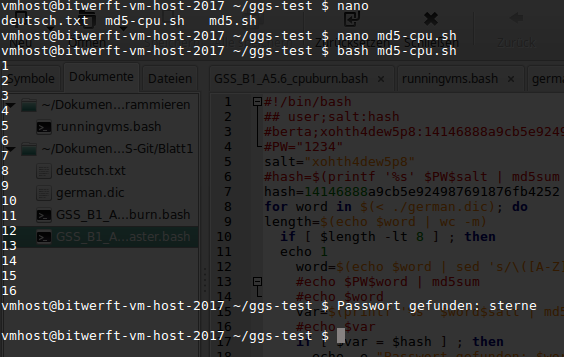
\includegraphics[scale=0.95]{Passwortgefunden.png} \\
Wenn der Salt nicht bekannt wäre, müsste nach einem Passwort in der maximalen Länge von Passwortlänge + Saltlänge gesucht werden.




\end{document}
